\documentclass[12pt]{beamer}

\usepackage[T2A]{fontenc}
\usepackage[utf8]{inputenc}
\usepackage[russian]{babel}
\usepackage{amsthm, amsmath, amssymb}
\usepackage{hyperref}
\usepackage{datetime}
\usepackage{cmap}
\usepackage{enumerate}
\usepackage{color}
\usepackage{picture}
\usepackage{graphicx}
\usepackage{tikz}
\usepackage{xcolor}
\usetikzlibrary{positioning,shadows,arrows}

\usepackage{bold-extra}

\def\EPS{\varepsilon}
\def\SO{\Rightarrow}
\def\EQ{\Leftrightarrow}
\def\t{\texttt}

\usetheme{Luebeck}
\usecolortheme{beaver}

\let\Tiny=\tiny
\useoutertheme{infolines}

\tikzset {
    fact/.style={rectangle, draw=none, rounded corners=1mm, fill=blue, drop shadow,
        text centered, anchor=north, text=white},
    new/.style={circle, draw=none, fill=orange, circular drop shadow,
        text centered, anchor=north, text=white},
    state/.style={circle, draw=none, fill=red, circular drop shadow,
        text centered, anchor=north, text=white},
    leaf/.style={rectangle, draw=black,
    minimum width=0.5em, minimum height=0.5em},
    cur/.style={circle, draw=none, fill=green, circular drop shadow,
        text centered, anchor=north, text=black},
    level distance=1.0cm, anchor=south
}

\begin{document}

\title{Blackout}

\author[]{
    Тонких Андрей \\
    Сазанович Никита \\
}
\institute[]{Санкт-Петербургский Академический университет}
\date{27 февраля 2017 года}

\frame{\titlepage}


\begin{frame}{Идея проекта}
    \begin{itemize}
        \item <1-> Динамичная multi-player action-арена с элементами РПГ, необычной физикой и системой взаимодействия заклинаний.
	      \item <2-> Социальные составляющие: рейтинги, достижения, лидеры
        \item[] <3-> \begin{center} 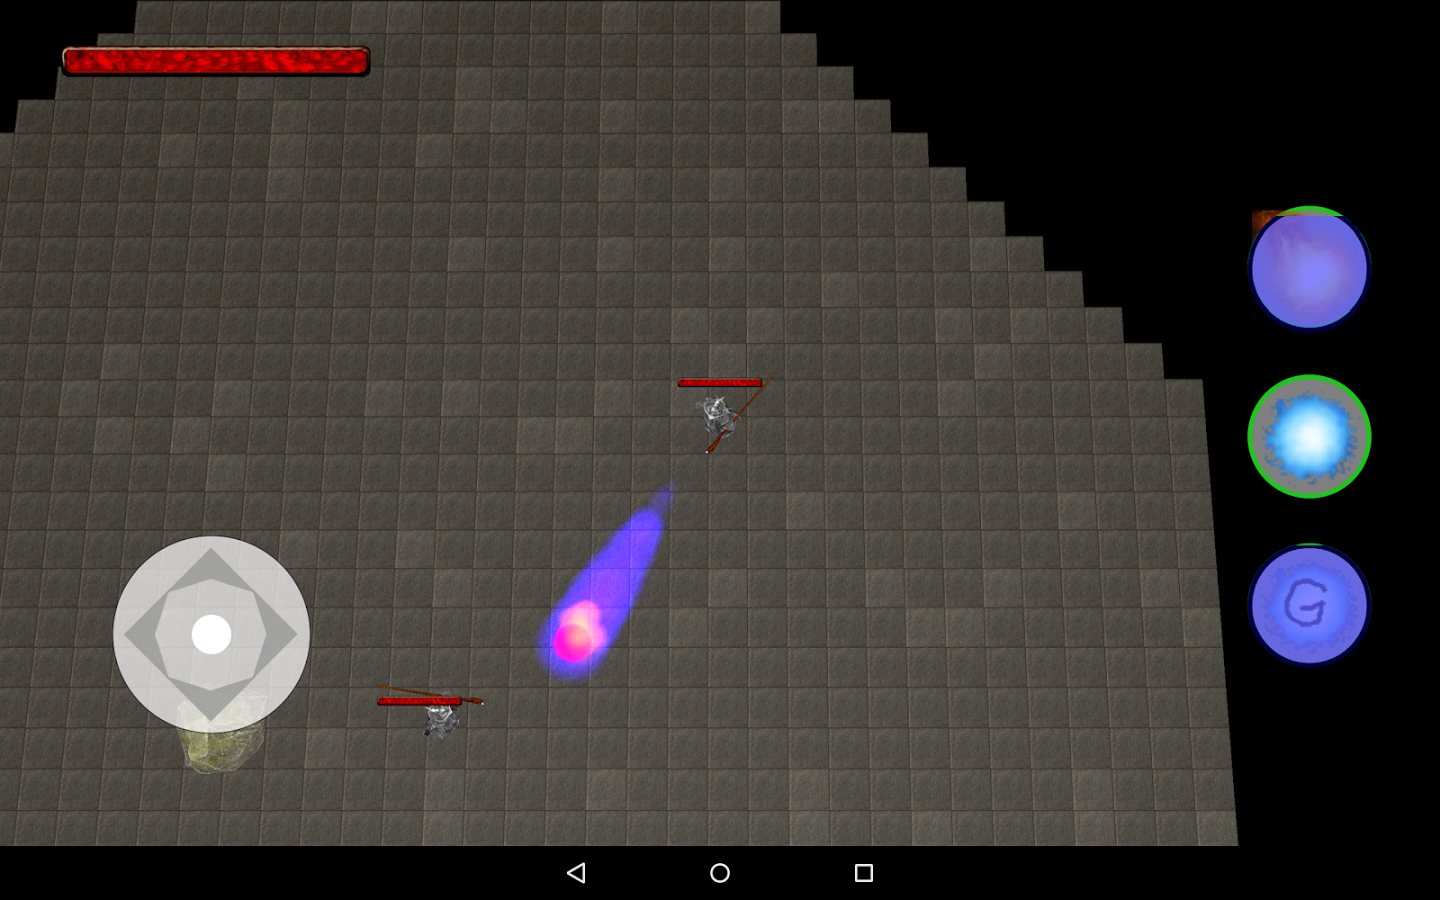
\includegraphics[width=230pt]{screenshot.png} \end{center}
    \end{itemize}
\end{frame}

\begin{frame} {Preview}
\end{frame}


\begin{frame} {Инструменты}
    \begin{itemize}
        \item Игровой движок libGDX
        \item Физический движок Box2D
        \item Иные инстерменты: Git, Travis CI, Blender, GIMP, Inkscape...
    \end{itemize}
\end{frame}



\begin{frame} {Архитектура}
\noindent\makebox[\textwidth]{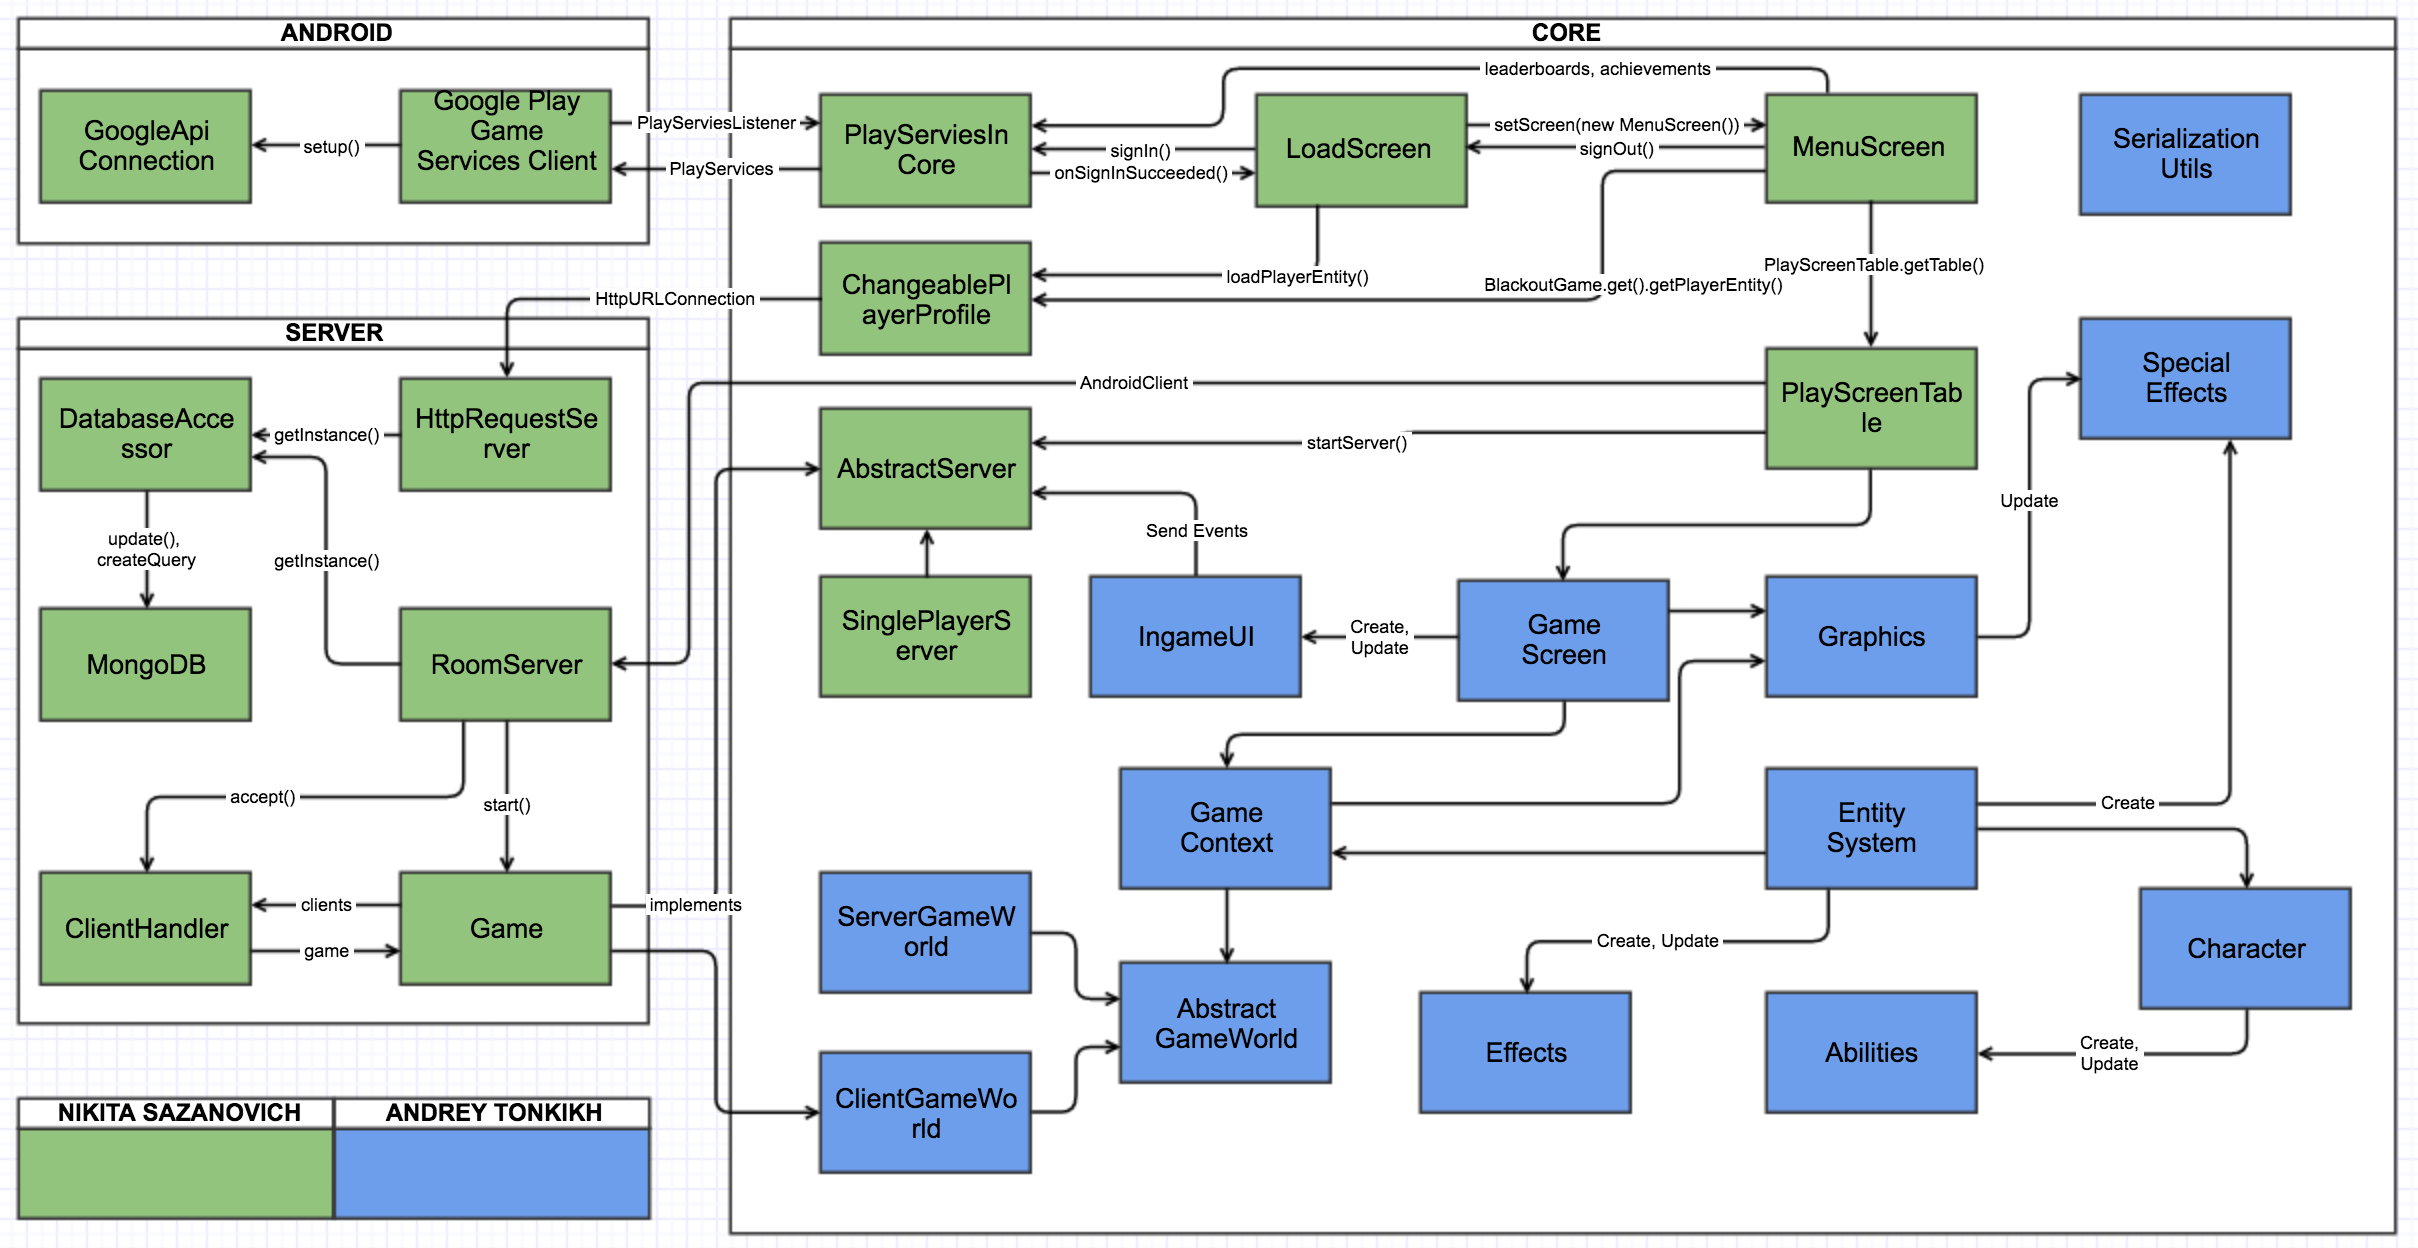
\includegraphics[width=\paperwidth]{architecture.png}}
\end{frame}


\begin{frame} {Android and Server}
    \begin{itemize}
        \item <1-> Возможности Android: Google Play Games Services
        \item <2-> Интерфейс меню приложения -- libGDX
        \item <3-> Выбор базы данных -- Saved Games (Google Drive) или local DB (MongoDB)?
        \item <4-> Написание сервера: для запросов пользователей HttpServer, для синхронизации игры Java Sockets
        \item <5-> Локальный сервер
    \end{itemize}
\end{frame}


\begin{frame} {Synchronization problems}
    \begin{itemize}
    	\item <1-> Какую модель выбрать: peer-to-peer (Google Play Game Services), один из игрков server или client-server?
	    \item <2-> Просчитывать ли дополнительно физику на клиенте?
	    \item <3-> Исследование networking-а: TCP$\rightarrow$UDP, custom serialization
    \end{itemize}
\end{frame}


\begin{frame} {Одиночная игра}
    \begin{itemize}
        \item[] <1-> Задача: одновременная поддержка одиночной и сетевой игры.
        \item[] <2-> \begin{center} 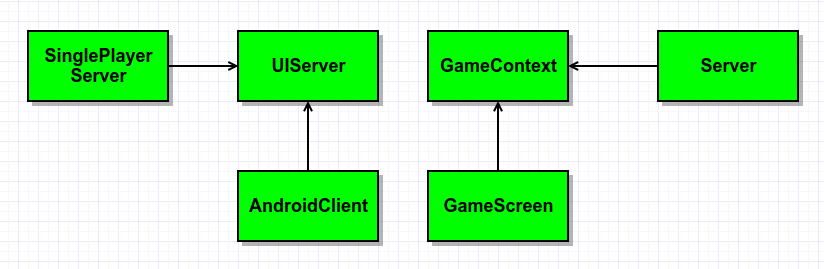
\includegraphics[width=300pt]{singleplayer.png} \end{center}
    \end{itemize}
\end{frame}


\begin{frame}{Графика и прочие ресурсы}
    \begin{itemize}
        \item <1-> Большое спасибо порталу http://opengameart.org/
        \item <2-> 2D $\rightarrow$ 3D
        \item <3-> Blender, Inkscape, GIMP
        \item <4-> Particle effects
    \end{itemize}
\end{frame}


\begin{frame}{Changelog}
    \begin{itemize}
        \item Новое заклинание: Gravity
        \item За счет своей сериализации и сжатия данных объем объем передаваемых по сети данных уменьшен в 4-5 раз
        \item Появилась система рейтинга
        \item Прогрессивная стоимость улучшений
    \end{itemize}
\end{frame}


\begin{frame}{Further improvements}
    \begin{itemize}
        \item <1-> Создание конкурентоспособного AI
        \item <2-> Добавление новых режимов и способностей
        \item <3-> Продуманный баланс
    \end{itemize}
\end{frame}


\begin{frame}{Results}
    \begin{itemize}
        \item <1-> Google play open alpha testing: \\ https://play.google.com/apps/testing/ru.spbau.blackout.android
        \item <2-> https://github.com/niksaz/blackout
    \end{itemize}

\end{frame}


\end{document}
